%\newpage
\section{Robustness and Adversarial Attack}

As explained in Section~\ref{sec:adversarialexample}, an adversarial example is an input that is close enough to, but with a different predicted label with, a correctly-predicted input. In most cases, the search for an adversarial example is formalised as an optimisation problem, in a form either the same as or similar with Equation (\ref{equ:advexpopt}). 

\subsection{Limited-Memory BFGS Algorithm}

%Szegedy et al 
Some researchers \cite{szegedy2014intriguing} noticed the existence of adversarial examples, and described them as ``blind spots'' in DNNs. They found that adversarial images usually appear in the neighbourhood of correctly-classified examples, which can fool the DNNs although they are human-visually similar to the natural ones. It also empirically observes that random sampling in the neighbouring area (see the template solution we provided in Section~\ref{sec:competitionresilience}) is not efficient to generate such examples due to the sparsity of adversarial images in the high-dimensional space.
%since the adversarial examples have low probability of occurrence, they cannot be found efficiently by sampling around correctly-classified inputs. 
Thus, they proposed an optimisation solution to efficiently search the adversarial examples. Formally, assume we have a classifier $f:\real^{s_1} \rightarrow \{1 \dots s_K\}$ that maps inputs to one of $s_K$ labels, and $\textbf{x} \in \real^{s_1}$ is an input, $t \in \{1 \dots s_K\}$ is a target label such that $t \neq \arg\max_l f_l(\textbf{x})$. Then the adversarial perturbation $\textbf{r}$ can be solved by

\begin{equation}
  \begin{array}{l}
    ~~~~~~\min ||\textbf{r}||_2 \\
  \textit{s.t.}~~\arg\max_{l} f_l(\textbf{x}+\textbf{r}) = t \\
  ~~~~~~~~\textbf{x}+\textbf{r} \in \real^{s_1}
  \end{array}
\end{equation}
%
% \begin{itemize}
%     \item Minimize $||\textbf{r}||_2$ subject to:
% \begin{enumerate}
%     \item $\arg\max_l f_l(x + r) =t$
%     \item $x + r \in \real^{s_1}$
% \end{enumerate}
% \end{itemize}
Since the exact computation is hard, an approximate algorithm based on the limited-memory Broyden–Fletcher–Goldfarb–Shanno algorithm (L-BFGS) is used instead. 
Furthermore, they observed that adversarial perturbations are able to transfer among different model structures and training sets, i.e., an adversarial image that aims to fool one DNN classifier also potentially deceives another neural network with different architectures or training datasets \cite{szegedy2014intriguing}.

% an adversarial example generated for one DNN classifier will likely be an adversarial example for another classifier with different architectures or training datasets.

\subsection{Fast Gradient Sign Method}

Fast Gradient Sign Method~\cite{DBLP:journals/corr/GoodfellowSS14} is able to find adversarial perturbations 
%(with untarget class) 
with a fixed $L_{\infty}$-norm constraint. FGSM conducts 
%very efficient to compute, which basically 
%is
a one-step modification to all pixel values so that the value of the loss function is increased under a certain $L_{\infty}$-norm constraint. 
%
The authors claim that the linearity of the neural network classifier leads to the adversarial images because the adversarial examples are found by moving linearly along the reverse direction of the gradient of the cost function. 
%
% They highlight that since the precision of an individual input feature is typically limited, e.g., digital images often use only 8 bits per pixel and therefore are precise up to $1/255$, it is unreasonable for a classifier to respond differently to two inputs if they only differ on each feature by an amount that is less than the level of precision. 
% %
% However, consider the dot product between a weight vector $w$ and an adversarial example $x' = x + r$: 
% \begin{equation*}
%     w^{T}x'=w^{T}x + w^{T}r
% \end{equation*}
% and let $r = \epsilon\ \text{sign} (w)$, the activation growth can be maximized this way. If $w$ has $n$ dimensions with elements having average magnitude $m$,  the activation growth is $\epsilon m n$, i.e. increases linearly with respect to the dimensionality of the problem, whereas $||\eta||_{\infty}$ remains less than $\epsilon$. Thus, for high-dimensional problems, FGSM can make many small changes to the input to produce a large difference in model output.
%
Based on this linear explanation, an efficient linear approach is proposed to generate adversarial images \cite{DBLP:journals/corr/GoodfellowSS14}. Let $\theta$ represents the model parameters, $\textbf{x},y$ denote the input and the label and $J(\theta, \textbf{x}, y)$ is the loss function. We can calculate adversarial perturbation $\textbf{r}$ by
\begin{equation}
    \textbf{r} = \epsilon\ \text{sign}\left(\nabla_{\textbf{x}} J(\theta, \textbf{x}, y)\right)
\end{equation}
%Using this method they are able to efficiently generate adversarial perturbations that lead to high rate of misclassification. 
A larger $\epsilon$ leads to a higher success rate of attacking, but potentially results in a bigger human visual difference. This attacking method has since been extended to a targeted and iterative version~\cite{KGB2016}.


\begin{algorithm}[!htbp]
\SetAlgoLined
$i \leftarrow 0$\\
$\textbf{x}^i$ is randomised such that $||\textbf{x}-\textbf{x}^i|| < d$\\
\Repeat{$i=n$}{
$\textbf{x}^{i+1} \leftarrow Clip_{\textbf{x},||\cdot||, d}(\textbf{x}^i + \epsilon \text{sign}(\nabla_{\textbf{x}}\mathcal{L}(\textbf{x}^i,y)))$\\
$i \leftarrow i+1$
}
\Return $\textbf{x}^n $, as an adversarial example.
\caption{$\functionname{PGDAttack}(f,\textbf{x}, y, ||\cdot||, d, n, \epsilon)$, where $f$ is the original model that the user wants to attack, $\textbf{x}$ is the sample to be attacked, $y$ is the true label of $\textbf{x}$, $||\cdot||$ is the norm distance, $d$ is the radius, $n$ is the number of iterations,  and $\epsilon>0$ is an attack magnitude. }
 \label{alg:pgdalgorithm}
\end{algorithm}


Algorithm~\ref{alg:pgdalgorithm} presents a pseudo code for PGD attack, where $Clip_{\textbf{x},||\cdot||, d}(\textbf{x}')$ is a clipping operation that projects any input $\textbf{x}'$ into  the norm ball centered at $\textbf{x}$ with radius $d$. 



\subsection{Jacobian Saliency Map based Attack (JSMA)}

A $L_0$-norm based adversarial attacking method is also presented by exploring the \emph{forward derivative} of a neural network \cite{JSMA}. Specifically, it utilises the Jacobian matrix of a DNN's logit output w.r.t. its input to identify those most sensitive pixels which then are perturbed to fool the neural network model effectively.
%
%which is used to highlight those features that the DNN's prediction is most sensitive to and are therefore most likely to cause miss-classification when perturbed. 
%
Let $c$ denote a target class and 
$\textbf{x} \in [0,1]^{s_1}$ represent an input image. JSMA will assign each pixel in $\textbf{x}$ a salient weight based on the Jacobian matrix. Each salient value basically quantifies the sensitivity of the pixel to the predicted probability of class $c$.
%
%The salient value captures, for each input dimension, the sensitivity of the output probability assigned to a class $c$. 
%
To generate the adversarial perturbation, the pixel with the highest salient weight is firstly perturbed by a \emph{maximum distortion parameter} $\tau > 0$. If the perturbation leads to a mis-classification, then JSMA attack terminates. Otherwise, the algorithm will continue until a mis-classification is achieved. When a maximum $L_0$-norm distortion $d > 0$ is reached, the algorithm also terminates. 
%or the input is  miss-classified. 
This algorithm is primarily to produce adversarial images that are optimized under the $L_0$-norm distance.
%JSMA is a $L_0$-norm target attacking method. 
JMSA is generally slower than FGSM due to the computation of the Jacobian matrix. %and aims to find an adversarial image that has a lower $L_0$-norm distance to the legitimate image.  

\subsection{DeepFool}

%Moosavi-Dezfooli et al 
In DeepFool, the researchers \cite{moosavi2016deepfool} introduce an iterative approach to generate adversarial images on any $L_p$ norm distance, for $p \in [1, \infty)$. In this work, they first show how to search adversarial images for an affine binary classifier, i.e., $g(\textbf{x}) = \text{sign}(\textbf{w}^T\cdot \textbf{x} + \textbf{b} )$. Given an input image $\textbf{x}_0$, DeepFool is able to produce an optimal adversarial image by projecting $\textbf{x}_0$ orthogonally onto the hyper-plane $\mathcal{F} = \{ \textbf{x} | \textbf{w}^T \cdot \textbf{x} +\textbf{b} =0\}$. Then this approach is generalised for a multi-class classifier: $\textbf{W} \in \real^{m \times k}$ and $\textbf{b} \in \real^k$. Let $\textbf{W}_i$ and $b_i$ be the $i$-th component of $\textbf{W}$ and $\textbf{b}$, respectively. We have 
\begin{equation*}
g(\textbf{x}) = \underset{i \in \{1 \dots k\}}{\text{argmax}}~g_i(\textbf{x}) \text{ where } g_i(\textbf{x}) = \textbf{W}_i^T\textbf{x} + b_i
\end{equation*}
For this case, the input $\textbf{x}_0$ is projected to the nearest face of the hyper-polyhedron $P$ to produce the optimal adversarial image, namely,
\begin{equation*}
    P(\textbf{x}_0) = \bigcap_{i=1}^k \{\textbf{x} | g_{k_0}(\textbf{x}) \geq g_{i}(\textbf{x})  \}
\end{equation*}
where $k_0 = g(\textbf{x}_0)$. We can see that $P$ is the set of the inputs with the same label as $\textbf{x}_0$. In order to generalise DeepFool to neural networks, the authors introduce an iterative approach, namely, the adversarial perturbation is updated at each iteration by approximately linearizing the neural network and then performing the projection. Please note that, DeepFool is a heuristic algorithm for a neural network classifier that provides no guarantee to find the adversarial image with the minimum distortion, but in practice, it is a very effective attacking method.

\subsection{Carlini \& Wagner Attack}

{\em  C\&W Attack} ~\cite{CW2016} is an optimisation based adversarial attack method which formulates finding an adversarial example as image distance minimisation problem such as $L_0, L_2$ and $L_\infty$-norm. Formally, it formulates the adversarial attack as an optimisation problem to minimise
\begin{equation}
{\mathcal{L}}(\textbf{r}) = ||\textbf{r}||_p + c \cdot F(\textbf{x} + \textbf{r}),
\end{equation} 
where $\textbf{x}+\textbf{r}$ is a valid input, and $F$ represents a surrogate function, such as $\textbf{x}+\textbf{r}$, which is able to fool the neural network when it is negative. The researchers directly adopt the optimiser Adam~\cite{kingma2014adam} to solve this optimisation problem. 
It is worthy to mention that C\&W attack can work on three distance metrics including $L_2$, $L_0$ and $L_{\infty}$ norms. 
%In particular for the $L_0$ case, an iterative algorithm identifies a subset of features having low impact on classification and are therefore not considered candidates for perturbation, this subset grows with each iteration, until its complement set is sufficiently small, giving a minimal feature subset salient to classification. At each iteration the feature $i$ selected for exclusion is the one that minimises $\nabla F(x +\textbf{r})_i \cdot \textbf{r}_i$.
%
A smart trick in C\&W Attack lies in that it introduces a new optimisation variable to avoid box constraint (image pixel need to be within $[0,1]$).  C\&W attack is shown to be a very strong attack which is more effective than JSMA~\cite{JSMA}, FGSM~\cite{DBLP:journals/corr/GoodfellowSS14} and DeepFool~\cite{moosavi2016deepfool}. It is able to find an adversarial example that has a significantly smaller distortion distance, especially on $L_2$-norm metric. 

	
% \subsubsection{Visual Adversarial Training}
% ~\cite{miyato2015distributional}: is primarily proposed for adversarial training so that the trained DNN classifier is more smooth and robust.  Its idea is to define a KL-divergence at an input image based on the model robustness to local perturbation around this image data-point. The most novelty lies on that it uses the KL divergence instead of the gradient with respect with the input $X$ (such as the one used in FGSM~\cite{goodfellow2014explaining}).


\begin{figure}
    \centering
    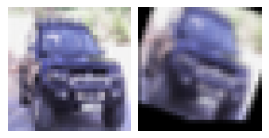
\includegraphics[width=0.6\textwidth]{images/deepLearning/AdversarialAttack/CIFAR10_rottran.png}
    \caption{Rotation-Translation: Original (L) `automobile', adversarial (R) `dog' from \cite{engstrom2017rotation}. {\em The original image of an `automobile' from the CIFAR-10 dataset is rotated (by at most $30^\circ$) and translated (by at most 3 pixels) results in an image that state-of-art classifier ResNet~\cite{he2016deep} classifies as `dog'.}}
    \label{fig:rottran}
\end{figure}

\subsection{Adversarial Attacks by Natural Transformations}\label{sec:naturalAdvAttacks}

Additional to the above approaches which perform adversarial attacks at a pixel level, research has been done on crafting adversarial examples by applying natural transformations.

\subsubsection{Rotation and Translation}

%Engstrom et al 
Some researchers \cite{engstrom2017rotation} argue that most existing adversarial attacking techniques generate adversarial images which appear to be human-crafted and less likely to be `natural'. It shows that DNNs are also vulnerable to some image transformations which are likely to occur in a natural setting. For example, translating or/and rotating an input image could significantly degrade the performance of a neural network classifier. Figure~\ref{fig:rottran} gives a few examples. 
%
Technically, given an allowed range of translation and rotation such as {\em $\pm3$ pixels $\times \pm 30^\circ$}, the attack in \cite{engstrom2017rotation} aims to find the minimum rotation and translation to cause a misclassification. To achieve such a purpose, in this work several ideas are explored including
\begin{itemize}
    \item a first-order iterative method using the gradient of the DNN's loss function,
    \item performing an exhaustive search by discretizing the parameter space,
    \item a worst-of-k method by randomly sampling $k$ possible parameter values and choosing the value that causes the DNN to perform the worst. 
\end{itemize}
%The experiments show that grid search performs best and can find adversarial examples for a significant number of images over   state-of-the-art classifiers.

\subsubsection{Spatially Transformed Adversarial Examples}

%Xiao et al 
Some researchers also
%Indeed an image may be translated by one pixel which would lead to a large $L_2$ distance, but the translated image would appear almost identical to a human. 
%They 
introduce
%therefore 
to produce uncontrived adversarial images via mortifying the pixel's location using spatial transformations instead of directly changing its pixel value \cite{xiao2018spatially}. The authors use the flow field to control the spatial transformations, which essentially quantifies the location displacement of a pixel to its new position. Figure~\ref{fig:stadvMNIST} gives a few examples. Using a bi-linear interpolation approach the generated adversarial example is differentiable w.r.t. the flow field, which then can be formulated as an optimisation problem to calculate the adversarial flow field.
Technically, they introduce a distance measure $L_{flow}(\cdot)$ (rather than the usual $L_p$ norm distance) to capture the local geometric distortion \cite{xiao2018spatially}. Similar to C\&W attack~\cite{CW2016}, the flow field is obtained by solving an optimisation problem in which the loss function is defined to balance between the $L_{flow}$ loss and adversarial loss.
%Comparing perceptual quality of spatially transformed adversarial images to adversarial images generated via other approaches in a quantitative manner is difficult due to the different measures used. However, 
Through human study, the attack in \cite{xiao2018spatially} demonstrates that adversarial examples based on such spatial transformation are more similar to original images in terms of human perceptibility, compared to those adversarial examples from $L_p$-norm based attacks such as FGSM~\cite{DBLP:journals/corr/GoodfellowSS14} and C\&W Attack~\cite{CW2016}.


\begin{figure}[t]
    \centering
    \begin{minipage}{0.24\textwidth}
        \centering
        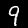
\includegraphics[width=\textwidth]{images/deepLearning/AdversarialAttack/UAN_MNIST_25sq_orig_9.png}
        \text{(a) Original:  `9'}
    \end{minipage}
    \begin{minipage}{0.24\textwidth}
            \centering
        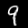
\includegraphics[width=\textwidth]{images/deepLearning/AdversarialAttack/UAN_MNIST_25sq_orig_9_perb_8.png}
        \text{(b) Adversarial: `8'}
    \end{minipage}
    \begin{minipage}{0.24\textwidth}
        \centering
        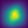
\includegraphics[width=\textwidth]{images/deepLearning/AdversarialAttack/x_flow.png}
        \text{(c) x-dimension}
    \end{minipage}
    \begin{minipage}{0.24\textwidth}
            \centering
        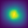
\includegraphics[width=\textwidth]{images/deepLearning/AdversarialAttack/y_flow.png}
        \text{(d) y-dimension}
    \end{minipage}
    \caption{Applying spatial transformation to MNIST image of a `9'~\cite{xiao2018spatially}. {\em the Image (a) on the left is the original MNIST example image of a `9', and image (b) is the spatially transformed adversarial version that a simple convolutional network \cite{papernot2018cleverhans} labels as `8'. Notice how minor the difference between the two images is - the `9' digit has been very slightly `bent' - but is sufficient for miss-classification. The flow-field that defines the spatial transformation is visualised in Image (c) (x-dimension) and Image (d) (y-dimension). The brighter areas indicate where the transformation is most intense - leftwards in the x-dimension and upwards in the y-dimension.}}
    \label{fig:stadvMNIST}
\end{figure}


\subsubsection{Towards Practical Verification of Machine Learning: The Case of Computer Vision Systems (VeriVis)}

The work in \cite{pei2017towards} introduces a verification framework, called VeriVis, to measure the robustness of DNNs on 
%`real-world' transformation functions. 
%
%Due to the often safety-critical nature of ML systems, it is imperative that DNNs can reliably classify corner-case inputs correctly. To verify this one would need to apply the system to all possible inputs - obviously not feasible. Indeed it is for exactly this reason that so much effort has been put into the generation of adversarial examples and their use for testing ML systems. However due to the extremely large domain space it is again not feasible to exhaustively generate all adversarial examples. Instead, the work in~\cite{pei2017towards} focuses on constraining a potential attacker to specific transformation functions having parameters within a specific range - for example consider the rotation function where the angle of rotation is within $\pm 10\degree $. Under these constrains, it can exhaustively test against \emph{all} transformed images. The key insight behind their approach is that ML systems work with discrete input - image pixels for example have integral coordinates taking integer values in $[0,255]$ and therefore rotation transformations having sufficiently similar angles will generate the same image. The \emph{critical} parameter domain for a given transformation and input is therefore defined as the finite subset of the parameter values that generate distinct output. This limits the domain of possible transformation functions to a finite amount (and indeed an amount which is only polynomial in the image size) thus allowing exhaustive testing. 
%
%The \textsc{VeriVis} framework specifies 
a set of twelve practical image transformations including reflection, translation, scale, shear, rotation, occlusion brightness, contrast, dilation, erosion, average smoothing, and median smoothing. Every transformation is controlled by a key parameter with a \emph{polynomial-sized} domain. Those transformations are exhaustively operated on a set of input images. Then the robustness of a neural network model can be measured.
%Thus let $\mathcal{T}(\cdot, c)$ be a transformation function parametric by $c \in C$ that transforms an input $x \in X$ to $x' = \mathcal{T}(x,c)$. A classifier $f: X \rightarrow Y$ can be thought of as \emph{Locally k-safe} for a given input $x \in X$ and transformation $\mathcal{T}(\cdot, c)$ if $f(\mathcal{T}(x,c)) \subseteq f(x, k)$ $\forall c \in C_{critical}$, where $f(x,k)$ is the set of top-k most likely predictions by $f$ for $x$, $C_{critical}$ is the critical parameter domain. A more challenging safety standard is \emph{Globally k-safe} requiring a classifier to be Locally k-safe $\forall x \in X$.
%
\textsc{VeriVis} is applied to evaluate several state-of-the-art classification models, which empirically reveals that all classifiers show a significant number of safety violations. %It is also argued that, 
%In comparison to the gradient-based adversarial techniques discussed above,
%\textsc{VeriVis} is capable of generating significantly more violations than gradient-based adversarial techniques.
%highlighting that gradient-based techniques may not be comprehensive. Furthermore the framework can be used to retrain classifiers using the found violations resulting in a more robust classifier having a greatly reduced number of safety-violations.



\subsection{Input-Agnostic Adversarial Attacks}\label{sec:inputAgnosticAdvAttacks}

A key characteristic of the above attacks lies in that an adversarial example is generated with respect to a specific input, therefore cannot be applied to other inputs. Thus some researchers show more interest in \emph{input-agnostic} adversarial perturbations.
%, and therefore may not perform adversarially when applied to another input example. %
%From the point of view of the malicious agent 

%for adversarial intent. Thus



\subsubsection{Universal Adversarial Perturbations}

The first method of input-agnostic adversarial perturbation was proposed by~\cite{moosavi2017universal}, called \emph{universal} adversarial perturbations (UAP), since UAP is able to fool a neural network on \emph{any} input images with high probability. 
%The first work on this line is proposed by Dezfooli et al \cite{moosavi2017universal}. With this approach \cite{moosavi2017universal} can generate UAPs that can fool state-of-the-art DNN classifiers with very high fooling ratios ($90\%+$ in some cases). In next, we review a few notable works in universal adversarial attacks.
%Technically, 
%Moosavi-Dezfooli et al
%\cite{moosavi2017universal} introduces UAPs and propose an algorithm for generating. The
%develope 
Let $\textbf{r}$ the the current perturbation. UAP iteratively goes through a set $D$ of inputs sampled 
%under the target 
from the input distribution $\mathcal{D}$. At the iteration for $x_i\in D$ it updates the perturbation $\textbf{r}$ as follows. First, it finds the minimal 
%(i.e. that with the smallest $L_2$-Norm) 
$\Delta \textbf{r}_i$ w.r.t. $L_2$-norm distance so that $x_i+\textbf{r}+\Delta\textbf{r}_i$ is incorrectly classified by neural network $\networks$. Then, it projects $\textbf{r} + \Delta\textbf{r}_i$ back into $L_p$-norm ball with a radius $d$ to enable that the generated perturbation is sufficiently small, i.e., let 
\begin{equation}
\begin{array}{1}
\textbf{r} = \arg\underset{\textbf{r}'}{\min} {||\textbf{r}' - (\textbf{r} + \Delta\textbf{r}_i) ||_2}\\
\text{s.t.~~} ||\textbf{r}'||_p \leq d.
\end{array}
\end{equation}
The algorithm will proceed until the empirical error of the sample set is sufficiently large, namely, no less than $1 - \delta$ for a pre-specified threshold $\delta$.


\subsubsection{Generative Adversarial Perturbations}

By training a universal adversarial network (UAN), some researchers \cite{hayes2018learning} generalised the C\&W attack in~\cite{CW2016} to generates input-agnostic adversarial perturbations. Assume that we have
%the data domain, $X$,  %classification set, %$\mathcal{Y}$, target DNN, %$g$, and 
a maximum perturbation distance $d$ and an $L_p$ norm, a UAN $\mathcal{U}_{\theta}$ randomly samples an input $z$ from a normal distribution and generates a raw perturbation $\textbf{r}$. Then it is scaled through $\textbf{w} \in [0, \frac{d}{||\textbf{r}||_p}]$ to have $\textbf{r}'=\textbf{w}\cdot \textbf{r}$. Then, the new input $\textbf{x}+\textbf{r}'$ needs to be checked with DNN $\networks$ to see if it is an adversarial example. 
%After that, $\textbf{r}'$ is added to an input $x$ and fed into $\networks$ with associated function $f$ to have %outputting 
%a prediction $f(x+\textbf{r}')$ for the adversarial image. 
The parameters $\theta$ are optimised by adopting a gradient descent method, similar to the one used by C\&W attack~\cite{CW2016}. 

%The experiments show that this UAN method generates UAPs that improve on the error rate, 1-$\delta$, from \cite{moosavi2017universal}.
%The UAN's architecture is composed of stacks of Deconvolution and Batch Normalisation layers, followed by a stack of fully-connected layers.

Later on, \cite{poursaeed2017generative} introduced a similar approach in\cite{hayes2018learning} to produce input-agnostic adversarial images. It first samples a random noise to input to UAN, and the output then is resized to meet an $L_p$ constraint which is further added to input data, clipped, and then is used to train a classifier. This method is different to~\cite{hayes2018learning} in two aspects. Firstly, it explores two UAN architectures including U-Net \cite{ronneberger2015u} and ResNet Generator \cite{johnson2016perceptual}, and concludes ResNet Generator works better in the majority of the cases. 
%The ResNet Generator architecture was  introduced 
%\cite{johnson2016perceptual} 
%for the task of \emph{image-transformation}, where the network outputs an image that has been transformed from the original input - typical transformations include colourisation, denoising or super-resolution. The architecture comprises of both up-sampling (deconvolution) and down-sampling (convolution) in residual blocks with batch normalisation and ReLU activation.
% 
Secondly, this work also trained a UAN by adopting several different classifiers, thus the proposed UAP can explicitly fool multiple classifiers, which is obtained by the below loss function:
%
\begin{equation}
    l_{multi-fool}(\lambda) = \lambda_1 \cdot l_{fool_1} + \dots + \lambda_m \cdot l_{fool_m}
\end{equation}
where $l_{fool_i}$ denotes the adversarial loss for classifier $i$, $m$ is the number of the classifiers, and $\lambda_i$ is the weight to indicate the difficulty of fooling classifier $i$.



\subsection{Practice}

%[xiaowei: here we need a code piece to do FGSM and PGD style attack on convolutional neural networks ]

First, we setup hyper-parameters (e.g., epsilon, steps, step size), device (e.g., CPU or GPU), and load training dataset (MNIST). Note that for FGSM: num-steps = 1 and  step-size = 0.031; for PGD-20: num-steps = 20 and step-size = 0.003.  
\begin{lstlisting}[language=Python]
import torch
import torch.nn as nn
import torch.nn.functional as F
import torch.optim as optim
from torchvision import datasets, transforms
import argparse
import time
import os
from torch.autograd import Variable

# Setup training parameters
parser = argparse.ArgumentParser(description='PyTorch MNIST Training')
parser.add_argument('--batch-size', type=int, default=128, metavar='N',
                    help='input batch size for training (default: 128)')
parser.add_argument('--test-batch-size', type=int, default=128, metavar='N',
                    help='input batch size for testing (default: 128)')
parser.add_argument('--lr', type=float, default=0.01, metavar='LR',
                    help='learning rate')
parser.add_argument('--no-cuda', action='store_true', default=False,
                    help='disables CUDA training')
parser.add_argument('--seed', type=int, default=1, metavar='S',
                    help='random seed (default: 1)')
parser.add_argument('--model-dir', default='./model-mnist-cnn',
                    help='directory of model for saving checkpoint')
parser.add_argument('--random', default=True,
                    help='random initialization for PGD')


# FGSM: num-steps:1 step-size:0.031   PGD-20: num-steps:20 step-size:0.003  
parser.add_argument('--epsilon', default=0.031,
                    help='perturbation')
parser.add_argument('--num-steps', default=1,
                    help='perturb number of steps, FGSM: 1, PGD-20: 20')
parser.add_argument('--step-size', default=0.031,
                    help='perturb step size, FGSM: 0.031, PGD-20: 0.003')

args = parser.parse_args(args=[]) 

if not os.path.exists(args.model_dir):
    os.makedirs(args.model_dir)
        
# Judge cuda is available or not
use_cuda = not args.no_cuda and torch.cuda.is_available()
#device = torch.device("cuda" if use_cuda else "cpu")
device = torch.device("cpu")

torch.manual_seed(args.seed)
kwargs = {'num_workers': 1, 'pin_memory': True} if use_cuda else {}

# Setup data loader
transform=transforms.Compose([
        transforms.ToTensor(),
        transforms.Normalize((0.1307,), (0.3081,))
        ])
trainset = datasets.MNIST('../data', train=True, download=True,
                   transform=transform)
testset = datasets.MNIST('../data', train=False,
                   transform=transform)
train_loader = torch.utils.data.DataLoader(trainset,batch_size=args.batch_size, shuffle=True,**kwargs)
test_loader = torch.utils.data.DataLoader(testset,batch_size=args.test_batch_size, shuffle=False, **kwargs)
\end{lstlisting}



\begin{lstlisting}[language=Python]
# Define CNN
class Net(nn.Module):
    def __init__(self):
        super(Net, self).__init__()
        # in_channels:1  out_channels:32  kernel_size:3  stride:1
        self.conv1 = nn.Conv2d(1, 32, 3, 1)
        # in_channels:32  out_channels:64  kernel_size:3  stride:1
        self.conv2 = nn.Conv2d(32, 64, 3, 1)
        self.fc1 = nn.Linear(9216, 128)
        self.fc2 = nn.Linear(128, 10)

    def forward(self, x):
        x = self.conv1(x)
        x = F.relu(x)
        x = self.conv2(x)
        x = F.relu(x)
        x = F.max_pool2d(x, 2)
        x = torch.flatten(x, 1)
        x = self.fc1(x)
        x = F.relu(x)
        x = self.fc2(x)
        output = F.log_softmax(x, dim=1)
        return output
\end{lstlisting}


Then we define the function for FGSM/PGD attack.
\begin{lstlisting}[language=Python]
def _pgd_whitebox(model,
                  X,
                  y,
                  epsilon=args.epsilon,
                  num_steps=args.num_steps,
                  step_size=args.step_size):
    out = model(X)
    err = (out.data.max(1)[1] != y.data).float().sum()
    X_pgd = Variable(X.data, requires_grad=True)
    if args.random:
        random_noise = torch.FloatTensor(*X_pgd.shape).uniform_(-epsilon, epsilon).to(device)
        X_pgd = Variable(X_pgd.data + random_noise, requires_grad=True)

    for _ in range(num_steps):
        opt = optim.SGD([X_pgd], lr=1e-3)
        opt.zero_grad()

        with torch.enable_grad():
            loss = nn.CrossEntropyLoss()(model(X_pgd), y)
        loss.backward()
        eta = step_size * X_pgd.grad.data.sign()
        X_pgd = Variable(X_pgd.data + eta, requires_grad=True)
        eta = torch.clamp(X_pgd.data - X.data, -epsilon, epsilon)
        X_pgd = Variable(X.data + eta, requires_grad=True)
        X_pgd = Variable(torch.clamp(X_pgd, 0, 1.0), requires_grad=True)
    err_pgd = (model(X_pgd).data.max(1)[1] != y.data).float().sum()
    return err, err_pgd

def eval_adv_test_whitebox(model, device, test_loader):
    # Ealuate model by white-box attack
    model.eval()
    robust_err_total = 0
    natural_err_total = 0

    for data, target in test_loader:
        data, target = data.to(device), target.to(device)
        # fgsm/pgd attack
        X, y = Variable(data, requires_grad=True), Variable(target)
        err_natural, err_robust = _pgd_whitebox(model, X, y)
        robust_err_total += err_robust
        natural_err_total += err_natural
    print('natural_accuracy: {:.2f}%'.format(0.01 * (10000-natural_err_total)))
    print('robust_accuracy: : {:.2f}%'.format(0.01 * (10000-robust_err_total)))
\end{lstlisting}


Finally, we load and attack the model.
\begin{lstlisting}[language=Python]
def main():
    model = Net().to(device)
    model.load_state_dict(torch.load(os.path.join(args.model_dir, 'final_model.pt')))
    eval_adv_test_whitebox(model, device, test_loader)
if __name__ == '__main__':
    main()
\end{lstlisting}











